\documentclass{article}
\setlength{\parindent}{0pt} 
\usepackage[margin=1in]{geometry}
\usepackage{titlesec}
\titlespacing*{\section}{0pt}{6pt}{3pt}
\titlespacing*{\subsection}{0pt}{5pt}{2pt}
\usepackage{graphicx} 
\usepackage{amsmath} 
\usepackage{bm}
\usepackage{amsmath}
\usepackage{amssymb}
\usepackage{amsthm}
\usepackage[title]{appendix}
\usepackage{mathrsfs}
\usepackage{amsbsy}
\usepackage{xcolor}
\newcommand{\red}{\textcolor{red}}
\usepackage{todonotes}
\usepackage{amsfonts}
 \usepackage{bm} 
\usepackage{booktabs} 
\usepackage{caption}  
\usepackage{float}    
\usepackage{threeparttable} 
\usepackage{algorithm}
\DeclareMathOperator{\OPT}{OPT}
\usepackage{algorithmicx}
\usepackage{algpseudocode}
\usepackage{listings}
\usepackage{enumitem}
\usepackage{chngcntr}
\usepackage{subcaption}
\usepackage{authblk}
\usepackage[T1]{fontenc}    
\usepackage{csquotes}     
\usepackage{diagbox}
\usepackage{tabularx}
\usepackage{xcolor}
\usepackage{colortbl}
\usepackage{comment}
\newcommand{\R}{\mathbb{R}}
\newtheorem{theorem}{Theorem}
\newtheorem{proposition}{Proposition}
\newtheorem{conjecture}{Conjecture}
\newtheorem{definition}{Definition}
\usepackage[numbers]{natbib} 
\bibliographystyle{abbrvnat} 

\newcommand{\bana}[1]{\green{[BANA: {#1}]}}
\newcommand{\lotan}[1]{\crimson{[LOTAN: {#1}]}}
\newcommand\toref{\red{[REF]}}
\newcommand\torefc[1]{\red{[REF: {#1}]}}
\renewcommand\todo[1]{{\red{TODO: {#1}}}}
\newcommand\tocite{\red{[CITE]}}
\newcommand\tocitec[1]{\red{[CITE: {#1}]}}


\title{\vspace{-5ex} Strategy-proof Allocation of Multiple Items between Two
Agents without Payments or Priors}
\author{
Auction Theory -- Course Project \\ submitted by: Bana Sadi (ID:206611477) and Lotan Amit (ID: 208800342)
}%(AAMAS 2010),}

\date{\vspace{-5ex}}
\begin{document}

\maketitle
\noindent

\textbf{Authors}: Mingyu Guo and Vincent Conitzer \\

\textbf{Published in:} Proc. of
9th Int. Conf. on Autonomous Agents and Multiagent Systems 2010

\section{Topic and Main Claim.}

The paper studies the allocation of m heterogeneous divisible items between two agents with additive valuations, in a setting where neither monetary transfers nor a prior distribution over valuations are available. The main claim is that the LIP mechanism (linear increasing-price) is a near-optimal solution to the problem of strategy-proof, payment-free allocation of two items between two agents, achieving a competitive ratio within about 1\% of the best possible strategy-proof mechanism; as the number of items grows, its competitiveness declines and provably converges to no better than the trivial even-split mechanism.

\section{Relation to Course}
The paper belongs to \emph{mechanism design without money}. The closest model
studied in the course is Moulin's strategy-proof mechanism for single-peaked
preferences \cite{moulin}: in both settings, payments are unavailable, so
strategy-proofness must come from the allocation rule alone. The main
difference is preference structure and objective. Moulin exploits
single-peaked preferences over a one-dimensional public alternative and
focuses on strategy-proofness itself; Guo and Conitzer consider additive
valuations over multiple divisible \emph{private} goods, where agents'
interests directly conflict, and ask how much social welfare can be
preserved under the strategy-proofness constraint measured via a
\emph{competitive ratio} against the efficient allocation.

The LIP mechanism's ``artificial currency'' and fixed increasing price
schedule has no counterpart in Moulin's model: although the currency is not
a real payment, it creates a trade-off between goods while preserving
strategy-proofness, yielding a better welfare guarantee than what a
median-style rule (unavailable here, since no consensus outcome exists) could
offer without allowing monetary transfers.

\section{Main Results}

The paper contains several theorems, but we focus on the first two: together
they show that a fully explicit, strategy-proof, payment-free, prior-free
mechanism exists whose performance is provably close to the best any such
mechanism could hope to achieve, so we treat them as the core of the paper.

There are $m>1$ divisible items and two agents $i \in \{1,2\}$. An allocation $o=(p_1,\dots,p_m)\in O$, $p_j\in[0,1]$, gives agent 1 a share $p_j$ of item $j$ and agent 2 the remaining $1-p_j$. Agent $i$'s type is a normalized additive valuation vector $\vec v^i=(v^i_1,\dots,v^i_m) \in V$, $v^i_j\ge 0$, $\sum_j v^i_j=1$, where $v^i_j$ is agent $i$'s value for the \textit{entirety} of item $j$, giving utility $u^i(\vec v^i,o)=\sum_j p^i_j v^i_j$ ($p^1_j=p_j$, $p^2_j=1-p_j$). A payment-free mechanism $M:V\times V\to O$ is \emph{strategy-proof} if truth-telling is dominant for both agents:
$$\forall i,\ \vec v_i,\vec v_i',\vec v_{-i}:\quad u^i(\vec v_i, M(\vec v_i,\vec v_{-i})) \ge u^i(\vec v_i, M(\vec v_i',\vec v_{-i})).$$

The \emph{first-best} mechanism $M^*(\vec v_1,\vec v_2)\in \arg\max_{o\in O}\sum_i u^i(\vec v_i,o)$ maximizes social welfare. When using $M^*$ as a benchmark it is assumed that agents bid truthfully although $M^*$ is generally \emph{not} strategy-proof. A strategy-proof mechanism $M$ is at least \textbf{$\alpha$-competitive} if
$$\sum_i u^i(\vec v_i, M(\vec v_1,\vec v_2)) \ \ge\ \alpha\sum_i u^i(\vec v_i, M^*(\vec v_1,\vec v_2)) \qquad \forall\, \vec v_1,\vec v_2,$$
where  $\alpha$ is called $M$'s \textit{competitive ratio}; the maximal possible $\alpha$ is called $M$'s \textit{maximal competitive ratio}.

\begin{theorem}
 The competitive ratio of any strategy-proof, payment-free, prior-free mechanism for allocating $m$ items between two agents is at most $0.841$, for every $m\ge 2$
\end{theorem}

Theorem 2 exhibits a mechanism that nearly meets this upper bound. The mechanism at the center of the paper is a \textbf{linear increasing-price (LIP)} mechanism. With probability $1/2$ agent $i$ is the ``dictator'' and receives one unit of artificial currency, which she spends against a fixed, publicly known, strictly increasing linear price schedule $f(x)=ax+b$ for each item ($a,b>0$; normalizing $\int_0^1 f(t)^{-1}dt=1$ pins down $b=a/(e^a-1)$, so a single parameter $a$ indexes the family, written $\mathrm{LIP}(a)$). Since $f$ is increasing, the dictator's optimal strategy is the greedy one: always buy the item with the best current value-to-price ratio and whatever proportion of an item she does not buy goes to the other agent

\begin{theorem}
 For $m=2$ items, and two agents, the mechanism LIP(2) has competitive ratio of at least $0.828$, and at most $0.829$.
\end{theorem}

\section{Proofs}
\subsection{Theorem 1}
\textbf{Step 1 -- reduction to two items.}
Suppose $M$ is strategy-proof for $m>2$ items with competitive ratio
$\alpha$. Restrict attention to profiles where both agents value items
$3,\ldots,m$ at $0$, and let $M'$ be $M$ run on reports
$(v_{i1},v_{i2},0,\ldots,0)$, keeping only the induced allocation of items
$1,2$. $M'$ is itself strategy-proof: any profitable deviation under $M'$
would be the same deviation, padded with zeros, under $M$, contradicting
$M$'s strategy-proofness. Since $\operatorname{CR}(M)=\inf_{v\in\mathcal V_m} W_M(v)/OPT(v)=\alpha$
and the restricted domain $\mathcal V_2'\subseteq\mathcal V_m$ is smaller,
$\operatorname{CR}(M')=\inf_{v\in\mathcal V_2'}W_M(v)/OPT(v)\ge\alpha$: restricting
the domain a mechanism must handle only \emph{relaxes} the constraints, so
$\alpha_2^*\ge\alpha_m^*$ for the best achievable ratios. An upper bound
proved for two items is therefore automatically an upper bound for all $m$.

\textbf{Step 2 -- discretizing.}
A two-item type is $(x,1-x)$, $x\in[0,1]$; fix $N=50$, $h=1/N$, and restrict
further to $\mathcal T=\{(ih,(N-i)h)\mid i=0,\dots,N\}$, identified with
integers $0,\dots,N$ (another domain restriction, so $\alpha_2^*\ge\alpha_{\mathrm{disc}}^*$
is preserved). A mechanism on $\mathcal T\times\mathcal T$ is now finitely
many variables $p^r_{jk}\in[0,1]$ ($r\in\{1,2\}$, $0\le j,k\le N$): the share
of item $r$ agent 1 gets when reports are $j,k$ (agent 2 gets $1-p^r_{jk}$).
This turns strategy-proofness, feasibility, and competitiveness into finitely
many \emph{linear} constraints.

\textbf{Step 3 -- strategy-proofness as linear constraints.}
Agent 1's utility from misreporting $j'$ when agent 2 reports $k$ is
$u_1(j;j',k)=j\,p^1_{j'k}+(N-j)\,p^2_{j'k}$, so strategy-proofness requires
$j\,p^1_{jk}+(N-j)\,p^2_{jk}\ge j\,p^1_{j'k}+(N-j)\,p^2_{j'k}$ for all
$j,j',k$, and symmetrically for agent 2.

\textbf{Step 4 -- competitiveness as linear constraints.}
Achieved welfare is $W(j,k)=j\,p^1_{jk}+(N-j)\,p^2_{jk}+k(1-p^1_{jk})+(N-k)(1-p^2_{jk})$;
first-best welfare is $\max\{j,k\}+\max\{N-j,N-k\}$ (each item entirely to
whoever values it more). $\alpha$-competitiveness on $\mathcal T$ is
$W(j,k)\ge\alpha(\max\{j,k\}+\max\{N-j,N-k\})$ for all $j,k$ -- linear in the
$p^r_{jk}$ and in $\alpha$.

\textbf{Step 5 -- solving the LP.} Maximizing $\alpha$ subject to Steps 3--4
and $0\le p^r_{jk}\le1$ is an LP; solving it numerically ($N=50$) gives
$\alpha^*\approx0.841$. Any strategy-proof mechanism on the full type space
induces a feasible LP point with at least its own ratio, so no strategy-proof
mechanism can exceed $0.841$. \emph{Caveat:} this is a computer-assisted
bound, not an analytic one, a fully hand-verifiable proof would need an
explicit dual-LP certificate of value $0.841$, which the authors note but do
not supply.

\subsection{Theorem 2}
\textbf{Step 1: Reduce the type space and identify the objective.}
By normalization, each agent's values sum to one, so we may write the two type vectors as $(x,1-x)$ and $(y,1-y).$

Since $\mathrm{LIP}(a)$ is symmetric across agents, we may assume without loss of generality that $1\ge x\ge y\ge 0.$

This is exactly the shaded triangular region in Fig.~\ref{fig:lip_triangle}; the discarded upper-left half of the unit square corresponds to profiles obtained by swapping the two agents.

Under $x\ge y$, item $1$ is valued more by agent $1$, while item $2$ is valued
more by agent $2$. Hence the first-best welfare is $\OPT(x,y)=x+1-y.$

Let $p_1(x,y)$ and $p_2(x,y)$ denote agent $1$'s expected shares of items $1$ and $2$, respectively, where expectation is over the fair coin flip that chooses the dictator. The resulting expected welfare is
\[
S(x,y)
=x\,p_1(x,y)+(1-x)\,p_2(x,y)
+y\bigl(1-p_1(x,y)\bigr)
+(1-y)\bigl(1-p_2(x,y)\bigr).
\]
Hence $\alpha(a)
= \min_{1\ge x\ge y\ge0} {S(x,y)}/({x+1-y}).$

The mechanism is also symmetric across the two items. Combining agent and item symmetry maps $(x,y)\mapsto(1-y,1-x),$ which reflects the feasible triangle across the line $x+y=1$ while preserving the competitive ratio. This explains the mirrored structure visible in Fig.~\ref{fig:lip_triangle}. In particular, on the diagonal $x=y$ the agents
have identical types, so symmetry gives $p_1(x,x)=p_2(x,x)=\frac12,$ and hence $S(x,x)=\OPT(x,x)=1.$

\textbf{Step 2: Fix the price schedule.}
Recall from Section~3 that under $\mathrm{LIP}(a)$, $f(t)=at+b$, and $b={a}/({e^a-1})$ Hence, for $a=2$, $b={2}/{e^2-1}\approx 0.313$.

\textbf{Step 3: Determine a dictator's allocation.}
Consider a dictator with type $(x,1-x)$. Let $t$ denote the amount of artificial currency she spends on item $1$, so $1-t$ is spent on item $2$. If both items are purchased in positive amounts, Lemma 1 implies that the terminal prices are proportional to the dictator's values. Since $f(t)+f(1-t)=a+2b,$ the proportionality condition gives $x={at+b}/({a+2b}),$ and therefore $t(x)=({x(a+2b)-b})/{a}.$ Clipping $t(x)$ to $[0,1]$ yields the three regimes of Claim 5 in the paper \cite{GuoConitzer2010}: 
\[
t(x)=
\begin{cases}
0, & x\le \dfrac{b}{a+2b},\\[2mm]
\dfrac{x(a+2b)-b}{a},
& \dfrac{b}{a+2b}<x<\dfrac{a+b}{a+2b},\\[3mm]
1, & x\ge \dfrac{a+b}{a+2b}.
\end{cases}
\]
For $a=2$, the two thresholds are approximately $0.119$ and $ 0.881.$
These are the dashed vertical and horizontal regime boundaries shown in Fig.~\ref{fig:lip_triangle}.

Let $q_j(x)$ denote the fraction of item $j \in \{1,2\}$ obtained by a dictator of type $(x,1-x)$. Since each agent is dictator with probability $1/2$, $p_j(x,y) =  q_j(x)/2 + \bigl(1-q_j(y)\bigr)/2.$

The spending regimes also explain the extreme ratio-one region in the figure.
If $x\ge0.881$ and $y\le0.119,$ then agent $1$, when dictator, spends entirely on item $1$, while agent $2$,
when dictator, spends entirely on item $2$. Thus either dictator induces the
first-best allocation, and ${S(x,y)}/{\OPT(x,y)}=1.$

\textbf{Step 4: Use monotonicity to bracket the minimum.}
The expected shares satisfy $p_1(x,y)$  is increasing in $x$ and decreasing in $y$ while $p_2(x,y)$ is decreasing in $x$ and increasing in $y$. This allows us to sandwich $\alpha(a)$ using a discretization. Fix a large $N$, step $h=1/N$, and grid points $x_i = ih$, $y_j = jh$ for $i,j = 0,\dots,N$. For each $0\le j\le i<N$, consider the cell $[x_i,x_i+h]\times[y_j,y_j+h]$. When $i=j$, only part of the square satisfies $x\ge y$; bounding the
entire square is conservative and therefore preserves the lower bound. 
For every feasible $(x,y)$ in such a cell, $x+1-y\le x_i+h+1-y_j.$ Moreover, the monotonicity of $p_1$ and $p_2$ gives the termwise lower
bound:
\[
S(x,y)\ge
x_i\,p_1(x_i,y_j+h)
+(1-x_i-h)\,p_2(x_i+h,y_j)
+y_j\bigl(1-p_1(x_i+h,y_j)\bigr)
+(1-y_j-h)\bigl(1-p_2(x_i,y_j+h)\bigr).
\]
Therefore,
\[
\alpha(a)
\ge
\min_{0\le j\le i<N}
\frac{
\begin{aligned}
&x_i\,p_1(x_i,y_j+h)
+(1-x_i-h)\,p_2(x_i+h,y_j)\\
&+y_j\bigl(1-p_1(x_i+h,y_j)\bigr)\\
&+(1-y_j-h)\bigl(1-p_2(x_i,y_j+h)\bigr)
\end{aligned}
}{
x_i+h+1-y_j
}.
\]

For the upper bound, every grid point in the triangle is itself a feasible type profile. Hence
\[
\alpha(a)
\le
\min_{\substack{0\le i,j\le N\\x_i\ge y_j}}
\frac{S(x_i,y_j)}{x_i+1-y_j}.
\]

Thus the continuous minimum is sandwiched between a rigorous cellwise lower bound and the minimum ratio attained on the grid.

\textbf{Step 5: Evaluate at $a=2$.}
Setting $a=2,$ and $b={2}/({e^2-1}),$ and evaluating the two bounds on a sufficiently fine grid gives $\alpha(2)\ge0.828$ and $\alpha(2)\le0.829.$

Therefore, $\boxed{0.828\le\alpha(2)\le0.829.}$
In particular, $\mathrm{LIP}(2)$ is at least $0.828$-competitive.




% % \begin{proof}[proof of Theorem 2]
% \textbf{Setup.}
% Recall $\mathrm{LIP}(a)$: with probability $\tfrac12$ each agent is the dictator and spends $1$ unit of artificial currency against the linear price schedule $f(t) = at+b$, where $b$ is fixed by the normalization $\int_0^1 \frac{1}{f(t)}\,dt = 1$, giving $b = \dfrac{a}{e^a-1}$.

% Let the two agents' type vectors be $(x,1-x)$ and $(y,1-y)$ with $1\ge x\ge y\ge 0$ (WLOG, by relabeling). A dictator with type $x$ either takes an item outright (if the marginal value/price ratios are too skewed), or, in the interior case, spends $t = {(x(a+2b)-b)}\slash{a}$
% % \[
% % t = \frac{x(a+2b)-b}{a}
% % \]
% units of currency on item $1$ and $1-t$ on item $2$.
% % , receiving proportions
% % \[
% % \frac{\ln(at+b)-\ln b}{a} \ \text{ of item 1}, \qquad \frac{\ln(a(1-t)+b)-\ln b}{a}\ \text{ of item 2}.
% % \]

% Let $p_1(x,y), p_2(x,y)$ denote agent $1$'s expected share of items $1,2$ respectively (mixing over which agent is the dictator, with probability $\tfrac12$ each). Define the achieved social welfare
% \[
% S(x,y) = x\,p_1(x,y) + (1-x)\,p_2(x,y) + y\big(1-p_1(x,y)\big) + (1-y)\big(1-p_2(x,y)\big),
% \]
% and the first-best welfare $x + 1 - y$ (agent $1$ gets item $1$, agent $2$ gets item $2$, since $x\ge y \implies 1-x\le 1-y$). The maximal competitive ratio of $\mathrm{LIP}(a)$ is then $\alpha(a) = \min_{1\ge x\ge y\ge 0} {S(x,y)}\slash {(x+1-y)}.$


% \textbf{Monotonicity.}
% $p_1(x,y)$ is increasing in $x$ and decreasing in $y$; $p_2(x,y)$ is decreasing in $x$ and increasing in $y$. This allows us to sandwich $\alpha(a)$ using a discretization.

% \textbf{Grid sandwiching.}
% Fix a large $N$, step $h=1/N$, and grid points $x_i = ih$, $y_j = jh$ for $i,j = 0,\dots,N$. Using the monotonicity of $p_1,p_2$, on each grid cell $[x_i,x_i+h]\times[y_j,y_j+h]$ the numerator $S(x,y)$ can be bounded below by evaluating $p_1,p_2$ at the worst corner of the cell for each term:
% % \[
% % \alpha(a) \;\geq\; \min_{0\le i,j< N}
% % \frac{
% % x_i\, p_1(x_i,y_j+h) + (1-x_i-h)\,p_2(x_i+h,y_j)
% % + y_j\big(1-p_1(x_i+h,y_j)\big) + (1-y_j-h)\big(1-p_2(x_i,y_j+h)\big)
% % }{x_i+h+1-y_j}.
% % \]

% \[
% \begin{aligned}
% \alpha(a) &  \;\geq\; \\
% \min_{0\le i,j<N}
%  & \frac{
% x_i\, p_1(x_i,y_j+h) + (1-x_i-h)\,p_2(x_i+h,y_j)
% + y_j\big(1-p_1(x_i+h,y_j)\big) + (1-y_j-h)\big(1-p_2(x_i,y_j+h)\big)
% }{x_i+h+1-y_j}.
% \end{aligned}
% \]
% Since every grid point $(x_i,y_j)$ is itself a feasible point of the continuous domain, evaluating the exact ratio there gives a valid upper bound: $\alpha(a) \;\leq\; \min_{0\le i,j\le N} 
% {S(x_i,y_j)}\slash {(x_i+1-y_j)}.$
% % \[
% % \alpha(a) \;\leq\; \min_{0\le i,j\le N} \frac{S(x_i,y_j)}{x_i+1-y_j}.
% % \]

% \textbf{Numerical evaluation at $a=2$.}
% With $b = \dfrac{2}{e^2-1}$, evaluating the lower-bound expression numerically (for sufficiently large $N$) yields $\alpha(2) \;\geq\; 0.828,$
% % \[
% % \alpha(2) \;\geq\; 0.828,
% % \]
% and evaluating the upper-bound expression yields $\alpha(2) \;\leq\; 0.829.$
% % \[
% % \alpha(2) \;\leq\; 0.829.
% % \]

% Since any lower bound on the maximal competitive ratio is itself a valid competitive ratio (the mechanism performs at least this well on every input, not just the sampled grid points), $\mathrm{LIP}(2)$ is at least $0.828$-competitive. Combined with the upper bound, $0.828 \;\le\; \alpha(2) \;\le\; 0.829.$
% % \[
% % 0.828 \;\le\; \alpha(2) \;\le\; 0.829.
% % \]

% \begin{proof}[proof of Theorem 2] (sketch)

% Normalization forces $v_1+v_2=1$, so agent 1's type is $(x,1-x)$ and agent 2's
% is $(y,1-y)$; since $LIP(a)$ is symmetric over the agents by construction we may
% assume $1\geq x\geq y\geq 0$ (the blank upper-left half of the square in Fig. \ref{fig:lip_triangle} is exactly the region this discards), under which the first-best welfare is exactly
% $x+1-y$. The problem is therefore the minimization of $S(x,y)/(x+1-y)$ over the shaded triangle of Fig. \ref{fig:lip_triangle}, where $S$ is the expected welfare under $LIP(a)$.
% Also note that $LIP(a)$ is symmetric over the items, and composing the two symmetries gives $(x,y) \mapsto (1-y,1-x)$, a reflection of the triangle across its anti-diagonal ($x+y=1$) that preserves the ratio; this is why every feature of Fig. \ref{fig:lip_triangle} appears twice.
% By Claim 3 we may take $\int_0^1 dt/f(t)=1$, which for $f(x)=ax+b$ forces
% $b=a/(e^a-1)$, leaving the single parameter $a$ ($b\approx 0.313$ at $a=2$).
% Since prices rise, the dictator buys greedily, and by Lemma 1 the stopping
% prices of any partly bought items are proportional to her valuations. As
% $f(t)+f(1-t)=a+2b$ regardless of $t$, the constant of proportionality is pinned
% down, giving Lemma 2: $x=(at+b)/(a+2b)$, i.e. $t=(x(a+2b)-b)/a$. Clipping $t$
% to $[0,1]$ yields Claim 5's three regimes (all-in on either item, or an interior
% split), with switches at $x=b / (a+2b) \approx 0./119$ and $x=(a+b) / (a+2b) \approx 0.881$ (the dashed lines of Fig. \ref{fig:lip_triangle}, vertical for agent 1, horizontal for agent 2),  and averaging over the coin flip gives
% $p_j(x,y)=\tfrac12 q_j(x)+\tfrac12(1-q_j(y))$ and hence $S(x,y)$ in closed form.

% Two regions are immediate: on the hypotenuse $x=y$ we have identical types, giving $p_1=p_2= \frac{1}{2}$, so $S=x+1-y=1$ and the ratio is 1; and the bottom-right box $x \geq 0.881, y \leq 0.119$ both agents are all-in on their own item, so either dictator produces the first-best allocation and the ratio is again 1 (bottom-right white box region of Fig. \ref{fig:lip_triangle}).

% Because $S$ involves logarithms of clipped affine expressions with regime
% switches in both $x$ and $y$, the minimum is not available in closed form, and
% we instead bracket it on a grid of step $h=1/N$. For the upper bound, the grid
% points are a subset of the triangle, so the minimum over them can only
% overestimate the true minimum; evaluating at $a=2$ gives $\leq 0.829$. For the
% lower bound we partition the triangle into cells $[x_i,x_i+h]\times[y_j,y_j+h]$,
% replace the denominator by its cell maximum $x_i+h+1-y_j$, and bound the
% numerator termwise: since the minimum of a sum is at least the sum of the
% minima, and since $p_1$ is increasing in $x$ and decreasing in $y$ while $p_2$
% is the reverse, each of the four terms of $S$ attains its cell minimum at a
% known corner ($(x_i,y_j+h)$ for $xp_1$ and $(1-y)(1-p_2)$, and $(x_i+h,y_j)$ for
% $(1-x)p_2$ and $y(1-p_1)$). Minimizing the resulting constant expression over
% all cells gives $\geq 0.828$ at $a=2$. As any lower bound on the maximal
% competitive ratio is itself an achieved competitive ratio, $LIP(2)$ is
% $0.828$-competitive, and at most $0.829$-competitive.

% \end{proof}

\section{Figure}

\begin{figure}[H]
    \centering
    \begin{minipage}[c]{0.62\textwidth}
        \centering
        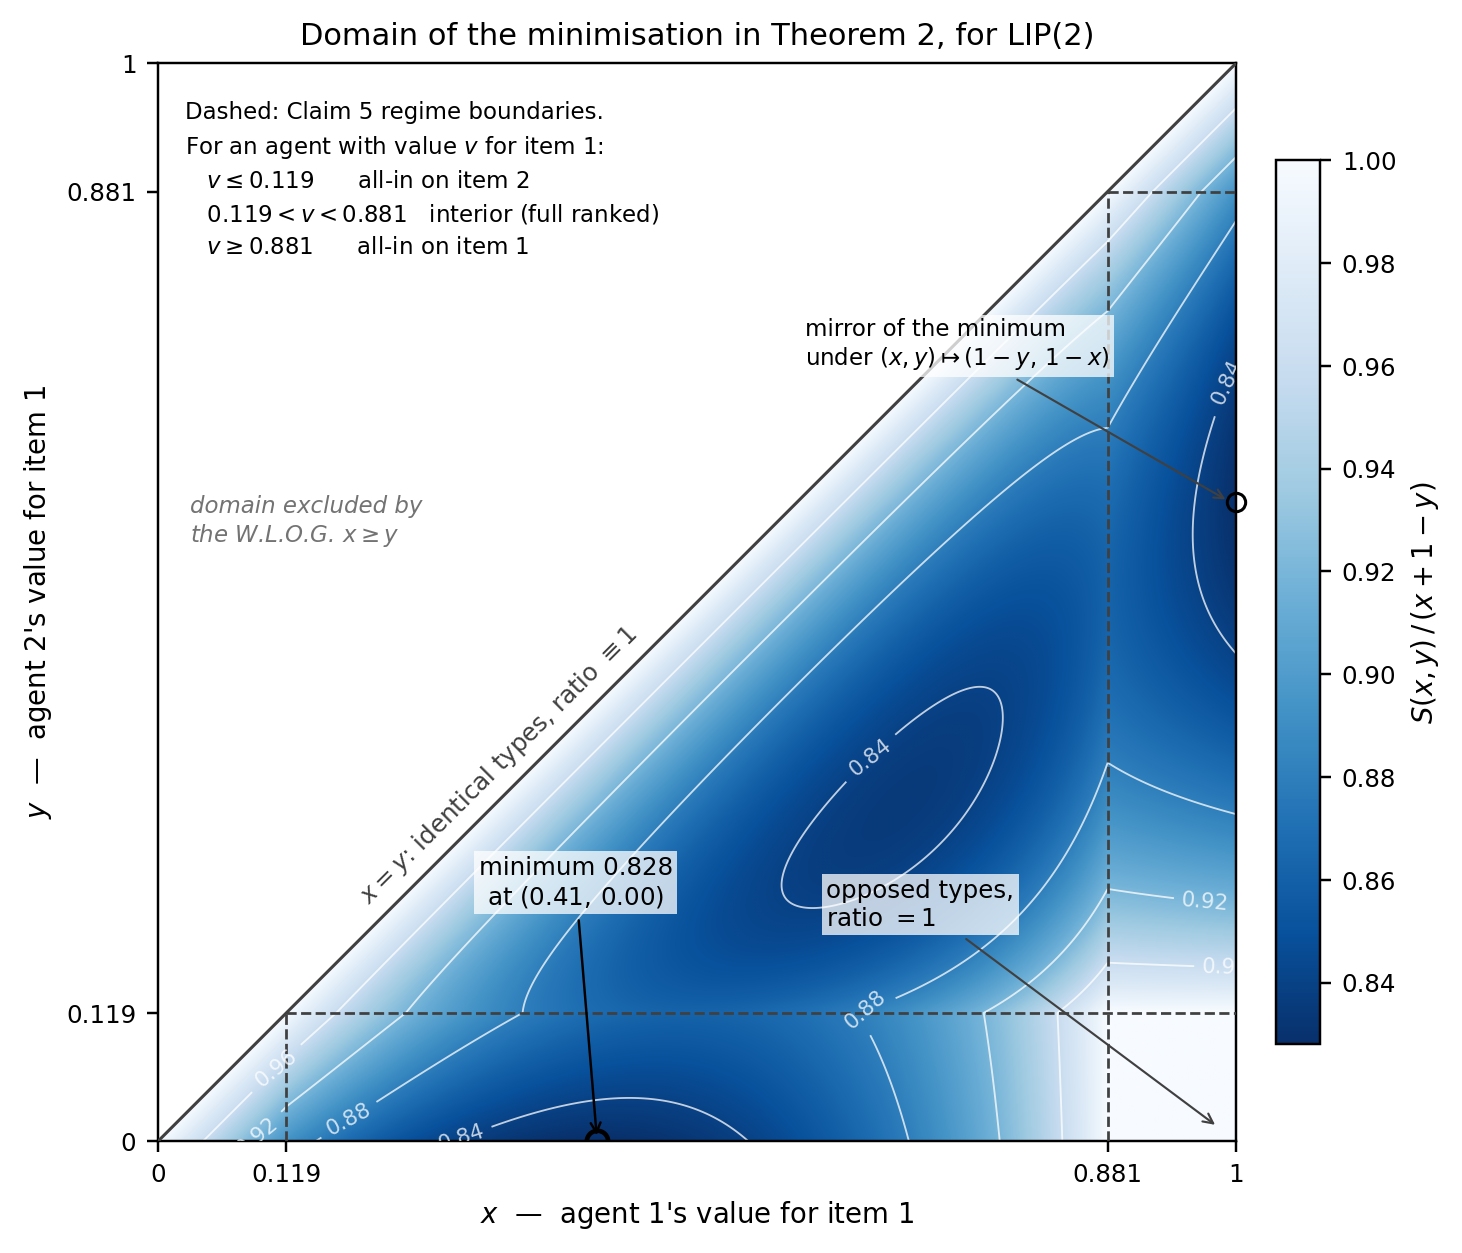
\includegraphics[width=\linewidth]{lip_triangle.png}
    \end{minipage}
    \hfill
    \begin{minipage}[c]{0.33\textwidth}
        % \caption{The feasible triangle $1\ge x\ge y\ge 0$ for Theorem 2, colored by
        % $S(x,y)/(x+1-y)$ at $a=2$. Dashed lines mark Claim 5's regime boundaries
        % ($0.119$, $0.881$); the marked minimum $0.828$ at $(0.41,0)$ matches the
        % lower bound derived in the proof, and the two labeled symmetric points
        % confirm that the diagonal ($x=y$) and anti-diagonal (opposed types) both
        % force ratio $1$.}

        \caption{The feasible triangle $1\ge x\ge y\ge 0$ for Theorem~2, colored by the competitive ratio $S(x,y)/(x+1-y)$ at $a=2$. The reduction to this triangular type space and the reflection symmetry across $x+y=1$ are explained in Step~1 of the proof. Dashed lines mark the regime boundaries from Claim~5, at approximately $0.119$ and $0.881$; their derivation from the dictator's optimal expenditure is given in Step~3. The white regions in which the ratio is exactly $1$ are discussed in Step~4. The marked worst-case value, approximately $0.828$ near $(0.41,0)$, is consistent with the rigorous grid bounds derived in Steps~5--6, which establish $0.828\le \alpha(2)\le 0.829$.}

        \label{fig:lip_triangle}
    \end{minipage}
\end{figure}
\section{Citations and Related Work}

\paragraph{An important citation: Procaccia and Tennenholtz \cite{Tennenholtz_Procaccia}.} Guo and Conitzer cite Procaccia and Tennenholtz to motivate assessing how much efficiency strategy-proof mechanisms can preserve without payments, even when exact efficiency is unattainable. Procaccia and Tennenholtz study facility location, minimizing total or maximum distance; Guo and Conitzer study private-goods allocation, maximizing total welfare. Thus, the former bound achieved cost relative to optimal cost from above, while the latter bound achieved welfare relative to optimal welfare from below. The environments also differ: a shared facility can simultaneously satisfy agents with identical preferred locations, whereas giving one agent more of a private good leaves less for the other. 


% The paper opens by framing its question as a continuation of Procaccia and Tennenholtz, \textit{Approximate Mechanism Design without Money} \cite{Tennenholtz_Procaccia}, credited with proposing competitive-ratio analysis as the right lens for asking how much is lost by removing payments, via facility location with single-peaked preferences. This matters twofold: it supplies the methodological paradigm (ask for the best approximation ratio, not a binary possibility/impossibility answer), and the authors use it to sharpen their own contribution since facility location admits a consensus outcome (median mechanisms work because agents aren't fundamentally in conflict), while private-goods allocation has none (every agent wants every item), which is exactly why an entirely different construction (artificial currency) was needed.

\paragraph{A paper that cites Guo and Conitzer.} \cite{han2011strategy} explicitly builds on this paper's model (``This model is first defined by Guo and Conitzer''), citing it as the source of the model and the LIP(2) benchmark their own results specialize and improve on. They tighten Theorem 1's bound with a cleaner proof, generalize to $n$ agents/$m$ items (no mechanism better than $\sim(1/m+\epsilon)$-competitive in general, or $4/\sqrt n$-competitive when $m\ge\sqrt n$), and, back in the two-agent setting, strengthen Theorem 4 by showing no \emph{swap-dictatorial} mechanism (not just increasing-price ones) exceeds $1/2+1/\sqrt{\lceil\log m\rceil}$.

\paragraph{A paper that, in our view, should have been cited.}  Hylland and Zeckhauser's \emph{The Efficient Allocation of Individuals to Positions} \cite{HyllandZeckhauser1979} provides a direct precedent for using artificial budgets and prices to allocate scarce resources without monetary transfers. Their pseudomarket assigns agents budgets for purchasing probabilities of receiving different positions. This connects closely to LIP's artificial currency, but highlights an important incentive difference: their market-clearing prices depend on reported preferences and can permit profitable manipulation, whereas LIP uses a predetermined price schedule and selects a dictator's preferred bundle from a fixed menu. Citing this work would place LIP within the earlier pseudomarket literature and clarify how its construction guarantees strategy-proofness.

% \section{Critique}

% The paper's conclusions are narrower than the headline result suggests. The
% restriction to two agents and additive valuations leaves preferences highly
% structured, and it is unclear how LIP behaves under complementarities or
% substitutes; the prior-free assumption buys robustness at the cost of never
% exploiting information about the population of agents. More importantly, the
% $0.841$ bound is a computer-assisted finite LP rather than an analytic
% characterization, with no dual certificate for independent verification --
% a limitation the authors acknowledge \cite{GuoConitzer2010}. There is also a
% conceptual tension in ``payment-free'' artificial currency: it never changes
% hands, but functions internally exactly as a pricing device, raising the
% question of how much of the mechanism's success is really about recreating
% prices rather than a genuinely different incentive principle. Finally, the
% decay to the trivial $1/2$ bound as items grow (Theorem 4) shows the approach
% does not scale, so the paper is best read as a positive result for a
% restricted environment, not a general solution to mechanism design without
% money.

\section{Critique}
The paper’s conclusions are narrower than the headline result suggests. The restriction to two agents and
additive valuations leaves preferences highly structured, and it is unclear how LIP behaves under complementarities or substitutes; the prior-free assumption buys robustness at the cost of never exploiting information
about the population of agents.
Also, the decay to the trivial $1/2$ bound as items grow (Theorem $4$) shows the approach does not scale, so
the paper is best read as a positive result for a restricted environment, not a general solution to mechanism
design without money.

\section{Plan for Part B}
We extend Guo and Conitzer's model by introducing complementarities between the two divisible goods. Agent $i$ has utility
\[
u_i(z_{i1},z_{i2})
=v_{i1}z_{i1}+v_{i2}z_{i2}+\epsilon z_{i1}z_{i2},
\qquad v_{ij}\geq0,\quad v_{i1}+v_{i2}=1,
\]
where the values $v_{ij}$ are private and $\epsilon\geq0$ is common and publicly known. For example, consider two firms sharing limited production and distribution capacity. A firm that receives additional production capacity can manufacture more units, but the benefit is greater when it also has distribution capacity to deliver those units to customers. Conversely, additional distribution capacity is more valuable when the firm can produce enough goods to use it. The term $\epsilon z_{i1}z_{i2}$ captures this complementarity: the marginal value of production capacity is $v_{i1}+\epsilon z_{i2}$, so it increases with the firm's allocation of distribution capacity.

\todo{add conjuncture}

\newpage

\section*{Part B: Extension}


% Section 1 of the Part B report: replication of Guo & Conitzer (2010).
% Paste into main.tex after the Part A sections.  Figure: results/figures/01_alpha_of_a.png.

\section{Replication of the paper's results}

\subsection{Why replicate}

Both headline numbers of the paper are computational. Theorem~1 ($\alpha\le0.841$ for every
strategy-proof mechanism) is the value of a linear program that the authors solved for one grid
size ($N=50$) without a dual certificate, and Theorem~2 ($0.828\le\alpha(\mathrm{LIP}(2))\le0.829$)
is a numerical sandwich evaluated ``for sufficiently large $N$'' whose $N$ is not reported. Neither
the code nor the intermediate quantities are available. Before extending the model we therefore
re-implemented every computation from the paper's formulas, checked that the stated numbers are
reproduced, and then asked the two questions the paper leaves open: how the LP bound depends on
the grid, and whether the price parameter $a=2$ is a good choice. All code is in the repository
(\texttt{core/lip.py}, \texttt{core/lp.py}), every number below is produced by
\texttt{notebooks/01\_replication.ipynb} and guarded by automated tests (\texttt{tests/}).

\subsection{Tools}

Python~3.14 with NumPy~2.5 and SciPy~1.18. Linear programs are solved with the HiGHS dual
simplex solver through \texttt{scipy.optimize.linprog} (sparse constraint matrices, default
tolerances $10^{-7}$), which also returns the dual multipliers we use in Section~2. The
one-dimensional optimisation over $a$ uses bounded Brent search
(\texttt{scipy.optimize.minimize\_scalar}). Everything else is vectorised NumPy; no Monte Carlo
sampling is used anywhere.

\subsection{Theorem 2: the competitive ratio of LIP(2)}

\paragraph{What the paper does.} With $f(t)=at+b$, $b=a/(e^a-1)$ and $Q(t)=\ln(1+at/b)/a$, Claim~5
gives the dictator's purchases in closed form, and $\alpha(a)=\min_{1\ge x\ge y\ge0}S(x,y)/(x+1-y)$.
The paper brackets this minimum on a uniform grid of step $h=1/N$: an upper bound from the exact
ratio at grid points, and a lower bound by replacing each of the four non-negative terms of
$S$ by its value at the worst corner of each cell (using that $p_1$ is increasing in $x$ and
decreasing in $y$, $p_2$ the reverse) and the denominator by its cell maximum.

\paragraph{What we did.} We implemented exactly this bracket (\texttt{lip.sandwich}) and
verified that a uniform grid reproduces the stated numbers only slowly: the upper bound is
$0.82815$ already at $N=50$, but the lower bound reaches $0.828$ only for $N\gtrsim 2\cdot10^4$,
i.e. $\sim4\cdot10^8$ cells. We therefore added \emph{adaptive refinement}
(\texttt{lip.sandwich\_adaptive}, \texttt{core/bracket.py}): starting from a $64\times64$ grid, a
cell is split into four only while its lower bound is below the best exact value found so far
minus a tolerance. Since every point of the triangle always lies in some leaf cell, the minimum
of the leaf lower bounds is a valid bound over the whole domain, exactly as in the paper's
argument. With tolerance $10^{-6}$ this needs about $2\cdot10^4$ cells and 30\,ms, and gives
\[
0.8281462\;\le\;\alpha(2)\;\le\;0.8281472,
\]
with the worst profile at $(x,y)\approx(0.4074,0)$: agent~2 wants only item~2, agent~1 mildly
prefers item~2 and, as dictator, buys most of it. The paper's $[0.828,0.829]$ is confirmed and
sharpened. We also reproduced Example~2 ($0.717$), the regime thresholds of Claim~5
($0.119$, $0.881$) and Figure~1 for $m=3,\ldots,100$ items (Theorem~3; intrinsic value $\theta(a)$
bracketed on a grid of $2000$ points, $a$ scanned on $0.01,\ldots,20$ as in the paper).

\subsection{Theorem 1: the LP upper bound}

\paragraph{What the paper does.} Types are restricted to $\{j/N\}$, $N=50$; variables
$p^r_{jk}\in[0,1]$ are agent~1's share of item $r$ at report profile $(j,k)$; strategy-proofness
and $\alpha$-competitiveness are linear constraints; the LP maximises $\alpha$.

\paragraph{What we did.} We built the same LP for arbitrary $N$ (\texttt{lp.solve\_sp\_lp}). Two
implementation choices are not in the paper and deserve a justification:
\begin{enumerate}
\item \emph{Local incentive constraints.} The paper's formulation has $O(N^3)$ constraints (every
  type against every misreport). Because a type's utility $x\,p^1+(1-x)\,p^2$ is \emph{affine}
  in the one-dimensional type $x$, incentive compatibility for all pairs is equivalent to the
  $O(N^2)$ constraints between \emph{adjacent} types: adding the two adjacent constraints for
  $x_j,x_{j+1}$ yields monotonicity of $p^1-p^2$ in the report, and monotonicity plus adjacent
  constraints imply every non-adjacent one by a telescoping argument. We verified on
  $N\le20$ that the full and the reduced LP have identical values (to $10^{-7}$), then used the
  reduced form, which is what makes $N=200$ feasible.
\item \emph{Symmetry.} We optionally impose the agent and item symmetries of Definition~2 as
  equalities. By the paper's Claim~1 this does not change the optimum (verified numerically),
  and it makes the solver several times faster and the solutions more structured.
\end{enumerate}
With $N=50$ the LP returns $\alpha=0.841225$, the paper's $0.841$.

\paragraph{New finding: the bound depends on the grid.} Restricting the type space only
removes constraints, so the LP value is a valid upper bound for \emph{every} $N$, and the
smallest value over $N$ is the one to quote. It decreases monotonically:
$0.8429$ ($N=40$), $0.8412$ ($50$), $0.8388$ ($80$), $0.8380$ ($100$), $0.8368$ ($150$),
$0.8363$ ($200$). A least-squares fit $\alpha_N\approx\alpha_\infty+c_1/N+c_2/N^2$ over $N\ge50$
gives $\alpha_\infty\approx0.8345$ (an extrapolation, not a bound). The paper's $0.841$ is thus
an artefact of $N=50$; the true gap between LIP and the best strategy-proof mechanism is less
than half of what the paper states.

\subsection{New finding: $a=2$ is not the best LIP mechanism}

The paper evaluates LIP only at $a=2$ and does not motivate the choice. Scanning $a$ with the
certified bracket (step $0.1$ on $[0.5,6]$, then Brent search on $[2.0,2.2]$) gives
\[
a^\star\approx2.1013,\qquad \alpha(a^\star)\approx0.82939\;>\;0.82815=\alpha(2).
\]
Figure~\ref{fig:alpha_a} explains the shape. Two restrictions of the minimisation give
rigorous upper bounds on $\alpha(a)$: along the anti-diagonal $x+y=1$ the ratio is the paper's
own intrinsic value $\theta(a)$ (Claim~8), and along the edge $y=0$ Lemma~2 gives
$Q(t)-Q(1-t)=\ln(\tfrac{x}{1-x})/a$, hence the closed form
\[
\beta(a)=\min_{b/(a+2b)\le x\le(a+b)/(a+2b)}\frac{1+\tfrac x2\big(1+\tfrac1a\ln\tfrac{x}{1-x}\big)}{1+x}.
\]
Numerically $\alpha(a)=\min\{\theta(a),\beta(a)\}$ to $10^{-6}$ on the whole scan: the edge
branch binds for $a<a^\star$, the anti-diagonal for $a>a^\star$, and the optimum is where the
two cross. Steeper prices (larger $a$) make the dictator buy a more balanced bundle, which helps
on the edge and hurts on the anti-diagonal.

\begin{figure}[H]\centering
\includegraphics[width=0.95\linewidth]{01_alpha_of_a.png}
\caption{Competitive ratio of LIP($a$) for additive valuations (certified brackets of width
$\le10^{-6}$, black) and the paper's intrinsic value $\theta(a)$ (dashed). The paper's $a=2$ (grey)
and the optimum $a^\star=2.1013$ (red). Right: zoom on the crossing of the two worst-case
branches.}
\label{fig:alpha_a}
\end{figure}

\subsection{Assumptions and caveats}

\begin{itemize}
\item \emph{Rigour of ``certified''.} The brackets are rigorous as mathematical inequalities but
  are evaluated in IEEE double precision, not interval arithmetic; rounding errors are of order
  $10^{-15}$, far below the reported $10^{-6}$ widths.
\item \emph{Grid parity.} LP values for small $N$ depend on whether particular rationals lie on
  the grid; we only draw conclusions from the monotone trend over $N\ge40$.
\item \emph{Extrapolation.} $\alpha_\infty\approx0.8345$ is a curve fit; the only proven
  statement is $\alpha\le0.8363$ ($N=200$).
\item \emph{Two worst-case lines.} That the minimiser of $S/(x+1-y)$ always lies on the edge or
  the anti-diagonal is verified numerically for $a\in[0.5,6]$, not proved; the values
  $\alpha(a)$ themselves do not depend on this.
\item \emph{Replication of Figure~1.} The paper's figure is read off visually; our curves agree
  with it qualitatively (ratios between $0.60$ and $0.73$, decreasing in $m$) but we could not
  compare individual values.
\end{itemize}




% \section{Motivation and model}
% Guo and Conitzer's LIP mechanism achieves strong welfare guarantees without payments when valuations are additive \cite{GuoConitzer2010}. Additivity excludes interactions between resources. Consider two firms sharing production capacity and distribution capacity: extra production capacity lets a firm manufacture more units, but those units are more valuable when the firm can also deliver them. Conversely, distribution capacity is more useful when there is output to distribute. A positive interaction term is therefore more realistic for this application than independent values for the two inputs. We investigate whether the original spending rule remains truthful, how to restore truthfulness, and what welfare the modified mechanism guarantees.

% There are two divisible goods, each of unit supply, and two agents with private types $x,y\in[0,1]$. A type-$x$ agent receiving fractions $(z_1,z_2)$ has utility $u_x^\epsilon(z_1,z_2)=xz_1+(1-x)z_2+\epsilon z_1z_2.$

% The coefficient $\epsilon$ is non-negative and publicly known. In the example, if $z_1$ denotes the fraction of production capacity allocated; the marginal value of production capacity is $x+\epsilon z_2$, which increases with distribution capacity. Agents maximize expected utility and only their types are reported; the resources and $\epsilon$ cannot be misreported. A full bundle has value $1+\epsilon$ for both agents. Dividing utilities by this common constant restores unit normalization and changes neither incentives nor welfare ratios.\\

% \textbf{The original menu and spending rule.} Retain LIP(2)'s artificial budget of 1 and its price schedule $f(t)=2t+b$, where $b=2/(e^2-1)$. Here $t$ is currency already spent on an item. For convenience, define
% \[
% Q(t)=\int_0^t\frac{ds}{2s+b}=\frac12\log\frac{2t+b}{b}.
% \]
% We use the notation $Q$ to denote the allocated-share formula. Spending $t$ buys fraction $Q(t)$, and $Q(0)=0$, $Q(1)=1$. Each agent is dictator with probability $1/2$. A dictator spending $t$ on good 1 receives $q(t)=(Q(t),Q(1-t))$; the other agent receives $1-q(t)$ componentwise. Under the original additive rule, report $r$ induces
% \[
% t_0(r)=\left[\frac{r(2+2b)-b}{2}\right]_0^1,
% \qquad [w]_0^1=\min\{1,\max\{0,w\}\}.
% \]
% Utilities are evaluated on the actual bundle in each dictator branch and then averaged. With nonlinear utilities, replacing this lottery by its expected bundle would change utilities and define another mechanism.

% \textbf{Research question.} Guo and Conitzer's LIP mechanism is strategy-proof for additive valuations \cite{GuoConitzer2010}. We ask what happens when a small complementary interaction is added while the original report-to-allocation rule is retained. 

% \textbf{Model.} There are two agents and two divisible goods, each of unit supply. Denote agent 1's vector type $(x, 1-x)$, agent 2's is $(y, 1-y)$ where $x,y \in [0,1]$. For a bundle $(z_1,z_2)$, a type-$x$ agent has utility
% \[
% u_x^\epsilon(z_1,z_2)=xz_1+(1-x)z_2+\epsilon z_1z_2,
% \qquad \epsilon\geq0.
% \]
% Types are private; $\epsilon$ is common and publicly known. Utilities are nonnegative, and agents maximize expected utility. 

% % For example, additional production capacity is more useful when a firm also has distribution capacity: its marginal value is $x+\epsilon z_2$. A full bundle has utility $1+\epsilon$ for every agent. Dividing all utilities by this common quantity would restore unit normalization without changing incentives or welfare ratios (utility-gain bounds would be divided by $1+\epsilon$).

% \textbf{Unchanged LIP(2).} Set $a=2$, $b=2/(e^2-1)$ and
% \[
% Q(t)=\frac12\log\frac{2t+b}{b},\qquad
%  t_0(r)=\left[\frac{r(2+2b)-b}{2}\right]_0^1,
% \]
% where $[w]_0^1=\min\{1,\max\{0,w\}\}$ and $Q(t)$ denotes the fraction
% of an item purchased by spending $t$ units of artificial currency. With probability $1/2$, each agent is selected as dictator. A dictator reporting $r\in[0,1]$ spends $t_0(r)$ on good 1 and the remaining budget on good 2, obtaining
% $q(t_0(r))=(Q(t_0(r)),Q(1-t_0(r)))$. The other agent receives the componentwise remainder. The rule uses the original additive spending calculation even when $\epsilon>0$. We average utilities of these actual bundles; nonlinear utility of an expected bundle would be a different mechanism.

% \begin{theorem}[Truthfulness is fragile, but manipulation is bounded]
% For every $\epsilon>0$, unchanged LIP(2) is not strategy-proof on this domain. For any true type, opposing report, and unilateral deviation, the gain in expected utility is at most
% \[
% \frac{\epsilon C}{2},\qquad
% C=Q(1/2)^2\approx0.513932.
% \]
% Thus the mechanism is $(\epsilon C/2)$-approximately strategy-proof, using the convention that no deviation gains more than this additive amount.
% \end{theorem}
% \begin{proof}
% For a dictator of true type $x$, define $F_x^\epsilon(t)=xQ(t)+(1-x)Q(1-t)+\epsilon P(t)$, where $P(t)=Q(t)Q(1-t)$. Since $Q'>0$ and $Q''<0$,
% \[
% P''(t)=Q''(t)Q(1-t)-2Q'(t)Q'(1-t)+Q(t)Q''(1-t)<0.
% \]
% The function $P$ is symmetric around $1/2$, hence $0\leq P(t)\leq P(1/2)=C$ and $P'(t)>0$ for $t<1/2$. Choose $x=1/4$. Its additive optimal spending satisfies $0<t_0(x)<1/2$ and $(F_x^0)'(t_0(x))=0$. Therefore $(F_x^\epsilon)'(t_0(x))=\epsilon P'(t_0(x))>0$. A slightly higher report induces slightly higher spending and strictly improves utility in the dictator branch. The agent's report has no effect in the other branch, so it improves expected utility as well.

% For the bound, $t_0(x)$ maximizes $F_x^0(t)$ over $[0,1]$. Any alternative spending $s$ therefore satisfies
% $F_x^\epsilon(s)-F_x^\epsilon(t_0(x))\leq\epsilon[P(s)-P(t_0(x))]\leq\epsilon C$.
% Multiplying by the probability $1/2$ of being dictator proves the claim, regardless of the other agent's report.
% \end{proof}

% \textbf{First-best welfare and a robustness guarantee.} Let $W_\epsilon^{\rm tr}(x,y)$ be expected total utility under truthful reports. Let $OPT_\epsilon(x,y)$ maximize total utility over all feasible allocations, without imposing incentive constraints. Randomization cannot increase this first-best benchmark, since an average cannot exceed the best realized welfare.

% \begin{proposition}[Exact benchmark]
% For every $x,y\in[0,1]$,
% \[
% OPT_\epsilon(x,y)=1+\max\{\epsilon,|x-y|\}.
% \]
% \end{proposition}
% \begin{proof}
% Utilities are nondecreasing, so a first-best allocation can assign every good in full. If agent 1 receives $(z_1,z_2)$ and agent 2 the remainder, total welfare is
% \[
% 1+(x-y)(z_1-z_2)+\epsilon\bigl[z_1z_2+(1-z_1)(1-z_2)\bigr].
% \]
% This is affine in each coordinate separately, so it attains a maximum at a corner of $[0,1]^2$ (move each coordinate to a maximizing endpoint). Giving both goods to either agent yields $1+\epsilon$; splitting them yields $1+x-y$ or $1-x+y$. Taking their maximum proves the formula. Thus complementarity favors concentrating goods when $\epsilon>|x-y|$, whereas sufficiently different additive preferences favor splitting them.
% \end{proof}

% \begin{theorem}[Truthful-report welfare]
% For every $\epsilon\geq0$ and every type profile,
% \[
% \frac{W_\epsilon^{\rm tr}(x,y)}{OPT_\epsilon(x,y)}
% \geq \frac{0.828}{1+\epsilon}.
% \]
% Moreover, the worst-case truthful-report ratio converges to zero as $\epsilon\to\infty$.
% \end{theorem}
% \begin{proof}
% The allocation rule does not change with $\epsilon$ and its interaction utilities are nonnegative. Hence Guo and Conitzer's Theorem 2 implies
% $W_\epsilon^{\rm tr}\geq W_0^{\rm tr}\geq0.828\,OPT_0$.
% Also $OPT_\epsilon\leq OPT_0+\epsilon$ and $OPT_0=1+|x-y|\geq1$. Therefore
% \[
% \frac{W_\epsilon^{\rm tr}}{OPT_\epsilon}
% \geq\frac{0.828\,OPT_0}{OPT_0+\epsilon}
% \geq\frac{0.828}{1+\epsilon}.
% \]
% For the asymptotic statement, take $x=y=0$. Either dictator obtains only good 2, and the other agent obtains only good 1. Welfare is exactly 1, while the optimum is $1+\epsilon$. Thus the worst-case ratio is at most $1/(1+\epsilon)$ and tends to zero. This statement concerns truthful reports, which cease to be dominant for $\epsilon>0$.
% \end{proof}

% \textbf{Strategic behavior can be computed exactly in one dimension.} For fixed true type $x$, the part of expected utility depending on the agent's report is $\tfrac12F_x^\epsilon(t_0(r))$. Since $t_0$ maps reports onto $[0,1]$, a best response is obtained by maximizing $F_x^\epsilon(t)$ on this interval. Its strict concavity follows from $Q''<0$ and $P''<0$, so the maximizing spending $t_\epsilon(x)$ is unique. An implementing report is
% \[
% r_\epsilon(x)=\frac{2t_\epsilon(x)+b}{2+2b}.
% \]
% Endpoint reports 0 and 1 can also implement endpoint spending. This best report is independent of the other agent's report and is therefore weakly dominant. The optimal spending is an endpoint when the derivative there has the appropriate sign; otherwise it is the unique root of
% \[
% (F_x^\epsilon)'(t)=
% \frac{x+\epsilon Q(1-t)}{2t+b}
% -\frac{1-x+\epsilon Q(t)}{2(1-t)+b}=0.
% \]
% The simulations use these dominant best responses rather than an assumed truth-telling equilibrium. Selecting $t_\epsilon(x)$ internally from a truthful report would define a different, strategy-proof mechanism; here we analyze strategic reports to the unchanged rule.

% \textbf{Numerical evaluation.} We evaluate 13 values of $\epsilon$ between 0 and 2 on a uniform grid of 1,001 types per agent (1,002,001 profiles for each $\epsilon$). Best-response spending is computed by endpoint checks and bracketed root finding. Expected utilities are evaluated analytically over the two dictator branches, with no Monte Carlo sampling. The exact benchmark is Proposition 1. We compare truthful LIP, LIP under dominant best responses, and deterministic equal division of both goods. The latter gives welfare $1+\epsilon/2$ independently of types and is strategy-proof because reports have no effect.

% \begin{center}
% \includegraphics[width=\linewidth]{results/results.pdf}
% \end{center}
% \vspace{-1em}
% \textbf{Figure 1.} Left: maximum sampled expected gain from unilateral manipulation, compared with the proved bound. This gain depends only on the manipulating agent's type. Right: minimum sampled welfare ratio, computed separately for truthful reports, dominant best responses, and equal division. Sampled extrema are numerical observations, not certificates for the continuous domain.

% \begin{center}
% \begin{tabular}{rrrrr}
% \toprule
% $\epsilon$ & Max. gain & Truthful LIP & Strategic LIP & Equal division\\
% \midrule
% 0 & 0.00000 & 0.82815 & 0.82815 & 0.50000\\
% 0.01 & 0.00009 & 0.83017 & 0.83082 & 0.50250\\
% 0.10 & 0.00658 & 0.84835 & 0.84028 & 0.52500\\
% 0.50 & 0.07993 & 0.66667 & 0.81002 & 0.62500\\
% 1.00 & 0.19625 & 0.50000 & 0.76515 & 0.75000\\
% 2.00 & 0.44429 & 0.33333 & 0.71528 & 0.66667\\
% \bottomrule
% \end{tabular}
% \end{center}
% The last three columns report minimum sampled welfare ratios. At $\epsilon=0$, the result lies in the original interval from 0.828 to 0.829. Positive manipulation gains appear for every sampled positive $\epsilon$, consistent with Theorem 1. The linear incentive bound is conservative for small interactions. Truthful-report performance initially improves, then deteriorates as complementarity becomes stronger; the lower bound in Theorem 2 is a robustness guarantee, not a prediction of monotonic empirical deterioration.

% Strategic reporting has no uniformly beneficial welfare effect in these experiments: at $\epsilon=0.1$ the worst sampled ratio is below the truthful counterpart, whereas at $\epsilon=0.5,1,2$ it is higher. The reported values are minima at potentially different profiles. We establish no general strategic-welfare guarantee from these observations.

% \textbf{Verification and limitations.} We independently checked the best-response solver against scalar optimization and repeated the experiment with 2,001 types per agent. Across the 13 interaction strengths, the largest change in a reported welfare minimum was $1.41\times10^{-7}$; the largest change in maximum manipulation gain was $8.04\times10^{-6}$. The analysis assumes a common known complementarity coefficient and the original one-dimensional report space. It does not cover private interaction coefficients or arbitrary substitutes. The contribution is a quantified robustness analysis of Guo and Conitzer's unchanged rule, including an exact benchmark and computable strategic behavior.


\bibliography{ref}

\end{document}
